\section{Ward Identities Part II, Interactions}
\subsection{Recap}
Last class we proved the Ward identity; a QFT with a continuous (``global'') symmetry has a current operator $j^\mu$ (in fact we can idnetify a current for each such symmetry that the theory has) which satisfies:
\begin{equation}
    \p_{y^\mu}\avg{\mathcal{T}\set{j^\mu(y), O_1(x_1), \ldots, O_n(x_n)}} = i\sum_{i=1}^n\delta^{d+1}(y - x_i)\avg{\mathcal{T}\set{O_1(x_1), \ldots, \Delta O_i(x_i), \ldots O_n(x_n)}}
\end{equation}
i.e. the current is conserved up to contact terms/operator insertions. At each coincident point, we measure the variation of the operator under that symmetry. One thing worth noting; so far symmetries that we have talked about are called ``global'' symmetries (to contrast what used to be called ``gauge symmetries'', which are not actually truly symmetries).

One example of this result is for the complex scalar field:
\begin{equation}
    S = -\int d^{d+1} \abs{\p\Phi}^2 + m^2\abs{\Phi}^2
\end{equation}
or alternatively two real fields $\Phi = \phi_1 + i\phi_2$. We can then consider:
\begin{equation}
    \p_{y^\mu}\avg{\mathcal{T}\set{j^\mu(y), \Phi^*(x_1), \Phi(x_2)}} = i\delta^{d+1}(y - x_1)\avg{\mathcal{T}\set{(-i)\Phi^*(x_1), \Phi(x_2)}} + i\delta^{d+1}(y - x_2)\avg{\mathcal{T}\set{\Phi^*(x_1), i\Phi(x_2)}}
\end{equation}
where we note that $\Delta \phi_1 = \phi_2$ and $\Delta \phi_2 = -\phi_1$ and so $\Delta \Phi = i\Phi$. 

\subsection{Commutators with Noether Charges}
Today we will derive a consequence of the Ward identities. We will integrate the Ward identity over the time component of $y$ (i.e. $y^\mu = (t, \v{y}), x^\mu_i = (t_i, \v{x}_i)$) over a small window around the time of the first operator, i.e. $t_1 - \e$ to $t_1 + \e$. Then, we integrate over all space, i.e. we consider:
\begin{equation}
    \int_{t_1-\e}^{t_1+\e}dt \int d^d\v{y}
\end{equation}
so, we will try to pick up the delta function/contribution from only the first operator.

If we do this, the RHS of the ward identity is very simple; a single delta function fires, and we get:
\begin{equation}
    \text{RHS} = i\avg{\mathcal{T}\set{\Delta O_1(x_1), O_2(x_2), \ldots, O_n(x_n)}}
\end{equation}
Now, let's see what happens to the LHS. First, look at the $\mu = 0$ component:
\begin{equation}
    \int d^d \v{y} j^0(t, \v{x}) = Q(t)
\end{equation}
For this component:
\begin{equation}
    \begin{split}
        \int_{t_1-\e}^{t_1+\e} \p_t\avg{\mathcal{T}Q(t)O_1(x_1)O_2(x_2)\ldots O_n(x_n)} = \left.\avg{\mathcal{T}Q(t)O_1(x_1)O_2(x_2)\ldots O_n(x_n)}\right|_{t = t_1-\e}^{t = t_1 + \e}
    \end{split}
\end{equation}
I.e. the integral is very simple (integral of a derivative!) Taking the $\e \to 0$ limit, the $Q(t)$ and $O_1(x_1)$ operator will be at the same time. But! Their order matters in the time ordering. In the first term, $Q$ is at a later time. In the second term, $Q$ is at an earlier time. In summary:
\begin{equation}
    \lim_{\e \to 0}\left.\avg{\mathcal{T}Q(t)O_1(x_1)O_2(x_2)\ldots O_n(x_n)}\right|_{t = t_1-\e}^{t = t_1 + \e} = \avg{\mathcal{T}[Q(t_1, O(x_1))]O_2(x_2)\ldots O_n(x_n)}
\end{equation}
What about the $\mu = i$ (Spatial) components? These vanish, as they are total derivatives and we integrate over all of space:
\begin{equation}
    \int d^d\v{y}\p_{y^i}(\ldots) = 0.
\end{equation}
Since this identity holds for any correlation function (i.e for any $O_2(x_2)\ldots O_n(x_n)$), it holds as an (equal-time) operator identity:
\begin{equation}
    \boxed{[Q, O_j(\v{x})] = i\Delta O_j(\v{x})}
\end{equation}
This is the path-integral derivation of the above relation. In PS6 we show this in a very different way (via canonical quantization).

\subsection{Our First Interacting Theory - Dimensional Analysis}
This next topic in the course is in some sense the most important; we will start to study interacting theories, introduce the concept of loops, and introduce the idea of renormalization/the renormalization group (arguably one of the most important developments in physics of the 20th century). We'll also study perturbation theory, which is how QFT makes most of its quantitative predictions. The relevant sections in Srednicki are 9, 12, 14.

Thus far, we've considered only Gaussian theories. Why? Because we were able to actually compute things/they are solvable. But if we want to go beyond this small set of free theories we know how to solve, we have to generalize.

To start, we consider the interacting theory (in $D = d + 1$ dimensions):
\begin{equation}
    S = -\int d^Dx \frac{1}{2}(\p\phi)^2 + \frac{1}{2}m^2\phi^2 + \frac{1}{3!}\lambda \phi^3
\end{equation}
Before any calculations, let's do some dimensional analysis. In relativistic QFT dimensional analysis is very easy, as $c = \hbar = 1$. So, $t \sim x$, and $E \sim \hbar \omega \sim \omega \sim \p_t \sim \frac{1}{t}$. In other words, we can measure everything in units of energy.

So, let's figure out the units of various things in the expression above. Since everything we add together has to have the same units, $m^2 \sim \p^2$. as $m^2\phi^2 \sim (\p\phi)^2$. So, we can write this as $m \sim E^1$ or $[m] = 1$. This of course we knew already from $E = mc^2 = m$. 

Let's look at $\lambda$; $\lambda \phi^3$ should have the same dimension as $m^2\phi^2$, so $\lambda \sim \frac{m^2}{\phi}$ and thus the dimension of $\lambda = 2[m] - [\phi] = 2-[\phi]$.

$\phi$ is not in general dimensionless. Let's find it's dimension. Since the action is dimensionless ($S \sim \hbar \sim 1$) this requires that $x^D \p^2\phi^2 \sim E^{2-D}\phi^2 \sim 1$ so $\phi \sim E^{\frac{D-2}{2}}$ or $[\phi] = \frac{D - 2}{2}$. Thus, $\lambda$ has dimensions $[\lambda] = 2 - [\phi] = \frac{6-D}{2}$.

As an example, in $D = 4$, $[\phi] = 1$ and $[\lambda] = 1$.

Not only is dimensional analysis useful for consistency check, we can often partially guess the answer to a question. For example, we recall the $m = 0$ Feynman Green's function in the free theory:
\begin{equation}
    G_F(p) = \frac{-i}{p^2}
\end{equation}
We will see that the leading correction to $G_F$ at order $\lambda^2$. By Lorentz invariance, it can only depend on $p$ through $p^2$, so:
\begin{equation}
    G_F(p) =  \frac{-i}{p^2} + C\frac{\lambda^2}{(p^2)^{\alpha}}
\end{equation}
by dimensional analysis, we can constrain the power $\alpha$:
\begin{equation}
    1 \sim \frac{p^{2(\alpha-1)}}{\lambda^2} \implies p^{\alpha-1} \sim \lambda \sim p^{\frac{6-D}{2}} \implies \alpha = \frac{8-D}{2}
\end{equation}
There is of course the order one number $O$ which we have to do a hard calculation to find, but we get a lot of information out of dimensional analysis (note that the dependency on $\lambda$ we can also get without doing the full calculation, as we will see).

\subsection{Our First Interacting Theory - Perturbative Corrections}
Let's find corrections to the connected two-point function:
\begin{equation}
    \bra{0}\mathcal{T}\phi(x)\phi(0)\ket{0}_C = \bra{0}\mathcal{T}\phi(x)\phi(0)\ket{0} - \bra{0}\phi(x)\ket{0}\bra{0}\phi(0)\ket{0}
\end{equation}
We have a nice path-integral representation for the above object:
\begin{equation}
    \bra{0}\mathcal{T}\phi(x)\phi(0)\ket{0}_C = \frac{\int \mathcal{D}\phi \phi(x)\phi(0)e^{iS}}{\int \mathcal{D}e^{iS}} - \frac{\int \mathcal{D}\phi(x)e^{iS}}{\int \mathcal{D}e^{iS}}\frac{\int \mathcal{D}\phi(0)e^{iS}}{\int \mathcal{D}e^{iS}}
\end{equation}
In the free theory, we found:
\begin{equation}
    G_{F, \lambda=0}(p) = \int d^Dx e^{-ip_\mu x^\mu}\avg{\phi(x)\phi(0)}_{\lambda=0} = \frac{-i}{p^2 + m^2 - i\e}
\end{equation}
We want to obtain corrections to the above. The strategy for these corrections will be very simple. We Taylor expand in $\lambda$ in the path integral:
\begin{equation}
    e^{iS} = e^{iS_0 + iS_{\text{int}}} \approx e^{iS_0}\left(1 + iS_{\text{int}} + \frac{i^2}{2}(S_{\text{int}})^2 + \ldots \right)
\end{equation}
We Taylor expand in the action (allowed, since its dimensionless)! But what do we mean to say ``expand in $\lambda$/$\lambda$ small''? We will take it to mean that it is small compared to the other energy scales in the problem, and we will see it manifest in the answer as the perturbative correction being valid above/below a certain momentum scale.

Our first observation; at $O(\lambda)$, there is no correction:
\begin{equation}
    \delta \avg{\phi(x)\phi(0)} = i\avg{\phi(x)S_{\text{int}}\phi(0)}_0 = \frac{i\lambda}{3!}\int d^dx'\avg{\phi(x)\phi^3(x')\phi(0)}_0 = 0
\end{equation}
where we use that the free field odd $n$-point functions vanish.

Therefore, let's look at the correction at $O(\lambda^2)$:
\begin{equation}
    \avg{\phi(x)\phi(0)}_\lambda \sim \frac{\int \mathcal{D}\phi \phi(x)\phi(0)(1 + iS_{\text{int}} + \frac{(iS_{\text{int}})^2}{2} + \ldots)e^{iS_0}}{\int \mathcal{D}\phi (1 + iS_{\text{int}} + \frac{(iS_{\text{int}})^2}{2} + \ldots)e^{iS_0}}
\end{equation}
We already noticed the linear terms gave zero. To properly normalize, we should divide the numerator and the denominator by the free field-theory normalization:
\begin{equation}
    \avg{\phi(x)\phi(0)}_\lambda = \frac{\int \mathcal{D}\phi \phi(x)\phi(0)(1 + iS_{\text{int}} + \frac{(iS_{\text{int}})^2}{2} + \ldots)e^{iS_0}/\int \mathcal{D}\phi e^{iS_0}}{\int \mathcal{D}\phi (1 + iS_{\text{int}} + \frac{(iS_{\text{int}})^2}{2} + \ldots)e^{iS_0}/\int \mathcal{D}\phi e^{iS_0}}
\end{equation}
So then we can truly express the numerator/denominator as free-field (time ordered) correlation functions:
\begin{equation}
    \avg{\phi(x)\phi(0)}_\lambda = \frac{\avg{\phi(x)\phi(0)\left(1 + \frac{i^2S_{\text{int}}^2}{2} + \ldots\right)}}{\avg{1 + \frac{i^2S_{\text{int}}^2}{2} + \ldots}} = \frac{\avg{\phi(x)\phi(0)}_0 + \frac{i^2}{2}\avg{\phi(x)S_{int}^2\phi(0)} + \ldots }{1 + \frac{i^2}{2}\avg{S_{\text{int}}}^2 + \ldots}
\end{equation}
So then:
\begin{equation}
    \avg{\phi(x)\phi(0)}_\lambda = \avg{\phi(x)\phi(0)}_0 + \frac{i^2}{2}\avg{\phi(x)S_{\text{int}}^2\phi(0)}_0 - \frac{i^2}{2}\avg{\phi(x)\phi(0)}_0\avg{S^2_{\text{int}}} + O(\lambda^3)
\end{equation}
Where the third term comes from $\frac{1}{1-x} \sim 1 + x$. Let's look at the first correction:
\begin{equation}
    \frac{i^2}{2}\avg{\phi(x)S_{int}^2\phi(0)} = -\frac{1}{2}\frac{\lambda^2}{(3!)^2}\int_{x_1}\int_{x_2}d^Dx_1d^Dx_2\avg{\phi(x)\phi^3(x_2)\phi^3(x_1)\phi(0)}_0
\end{equation}
which is an 8-point function in the free theory, which can be computed via Wick contractions!

There are many such contractions. But before we go there, note that there are contractions that will cancel with the other terms. Namely, the contractions where $\phi(x)$ gets contracted with $\phi(0)$ will cancel and not contribute to the final answer. Let's look at these. First, there is the case where we contract all pairs of $\phi(x_2)$s with $\phi(x_1)$s, which gives:
\begin{equation}
    G(x)G(x_1 - x_1)^3
\end{equation}
\begin{center}
    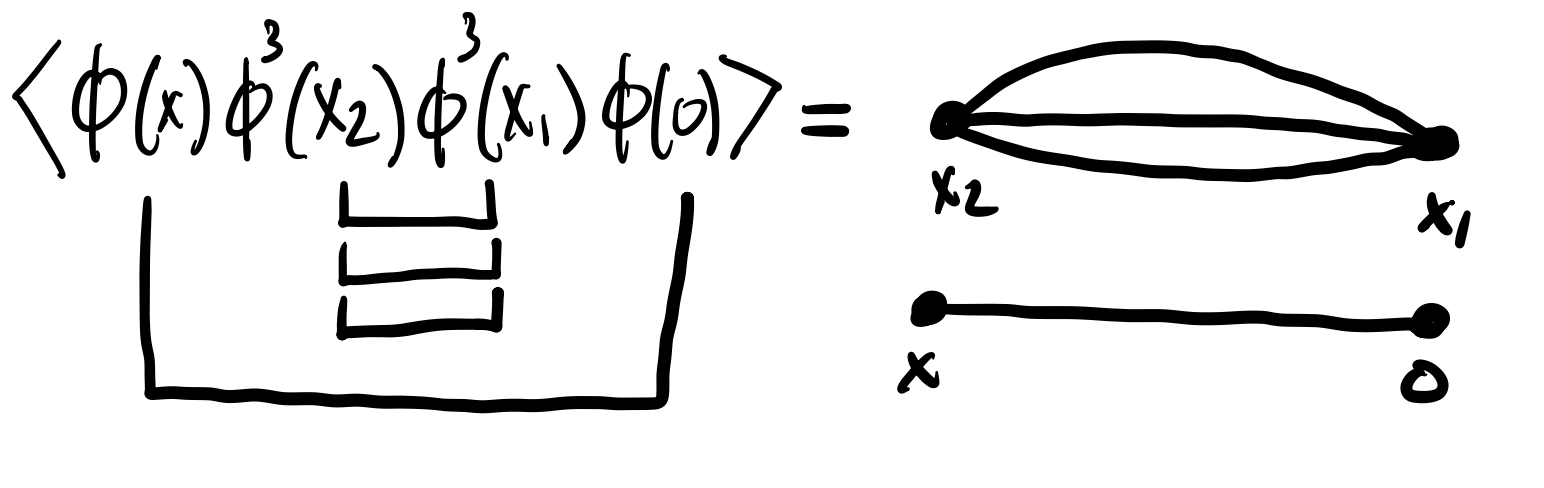
\includegraphics[scale=0.4]{Lectures/Figures/lec11-diag1.png}
\end{center}

The only other option is where we contract two $\phi(x_2)$s together, contract two $\phi(x_1)$, and finally contract one $\phi(x_1)$ with $\phi(x_2)$, which gives:

\begin{equation}
    G(x)G(0)^2G(x_2 - x_1)
\end{equation}

\begin{center}
    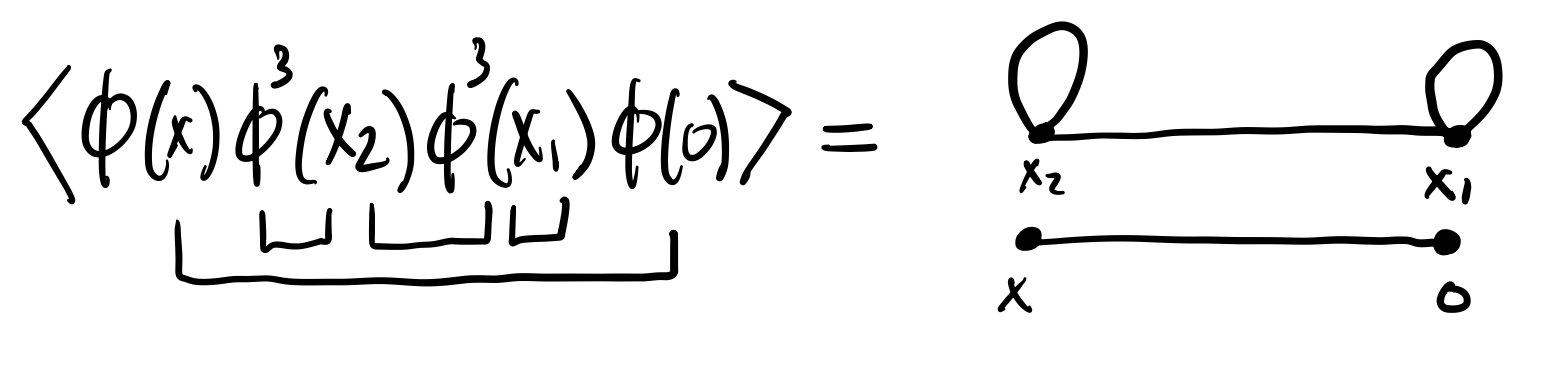
\includegraphics[scale=0.4]{Lectures/Figures/lec11-diag2.png}
\end{center}

These are a special type of diagram, because if we look at the $\avg{\phi(x)\phi(0)}_0\avg{S_{\text{int}}^2}_0$ term we will see they get exactly cancel. These diagrams are sometimes called ``bubble diagrams'' because there are bubbles/parts of the diagram that are separate from the main propagator (i.e. diagrams of the form $G(x) \cdot (\text{stuff})$\footnote{Luca - ``This is the formal definition.''}). Although we saw a specific example here, it is in fact generally true that they get cancelled from $\frac{1}{\int \mathcal{D} \phi e^{iS}}$.

What we are left with is:
\begin{equation}
    \avg{\phi(x)\phi(0)}_\lambda = \avg{\phi(x)\phi(0)}_0 + \frac{i^2}{2}\left.\avg{\phi(x)S^2_{\text{int}}\phi(0)}\right|_{\text{non-bubble}}
\end{equation}
Which contractions are left? Qualitatively, three. The first is where we contract $\phi(x)$ with a $\phi(x_2)$, $\phi(0)$ with a $\phi(x_1)$, and then pair up the remaining $\phi(x_2)$s with $\phi(x_1)$s, which gives:
\begin{equation}
    G(x - x_2)G(x_2 - x_1)^2 G(x_1)
\end{equation}
\begin{center}
    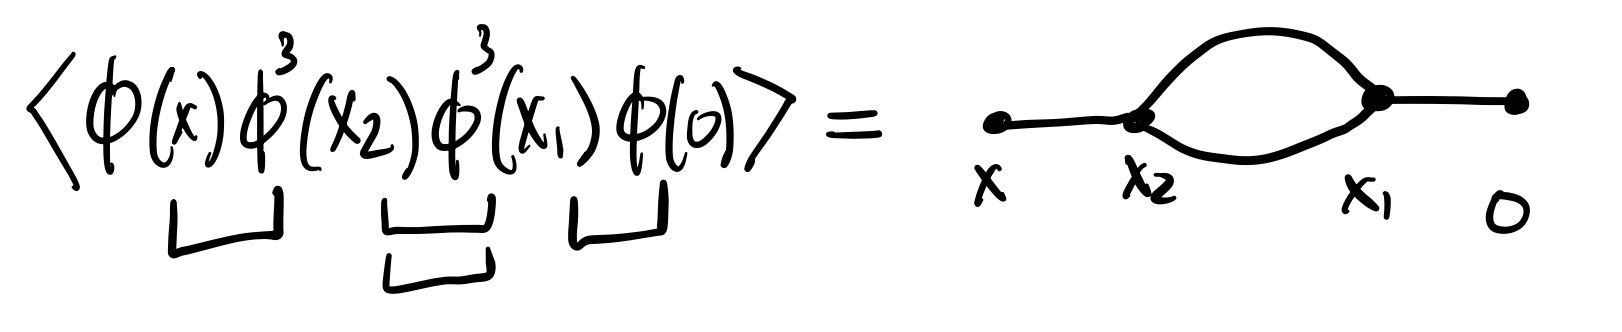
\includegraphics[scale=0.4]{Lectures/Figures/lec11-diag3.png}
\end{center}
The second is where we contract $\phi(x)$ with $\phi(x_2)$, and $\phi(0)$ is also contracted with $\phi(x_2)$. Then, we contract the remaining $\phi(x_2)$ with one $\phi(x_1)$ and two $\phi(x_1)$s together. This gives:
\begin{equation}
    G(x - x_2)G(x_2 - x_1)G(0)G(x_2)
\end{equation}
\begin{center}
    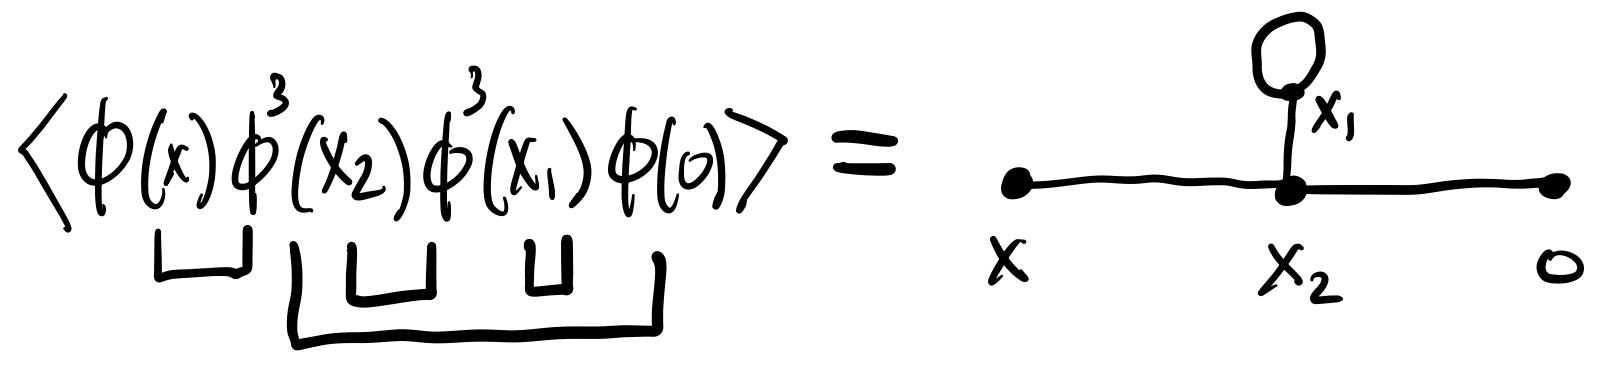
\includegraphics[scale=0.4]{Lectures/Figures/lec11-diag4.png}
\end{center}
Finally, in the last contraction we keep the left and right halves separate; contract $\phi(x)$ with a $\phi(x_2)$, $\phi(0)$ with $\phi(x_1)$, and $\phi(x_2)$s together and $\phi(x_1)$s together. This gives:
\begin{equation}
    G(x - x_2)G(0)^2 G(x_1)
\end{equation}
\begin{center}
    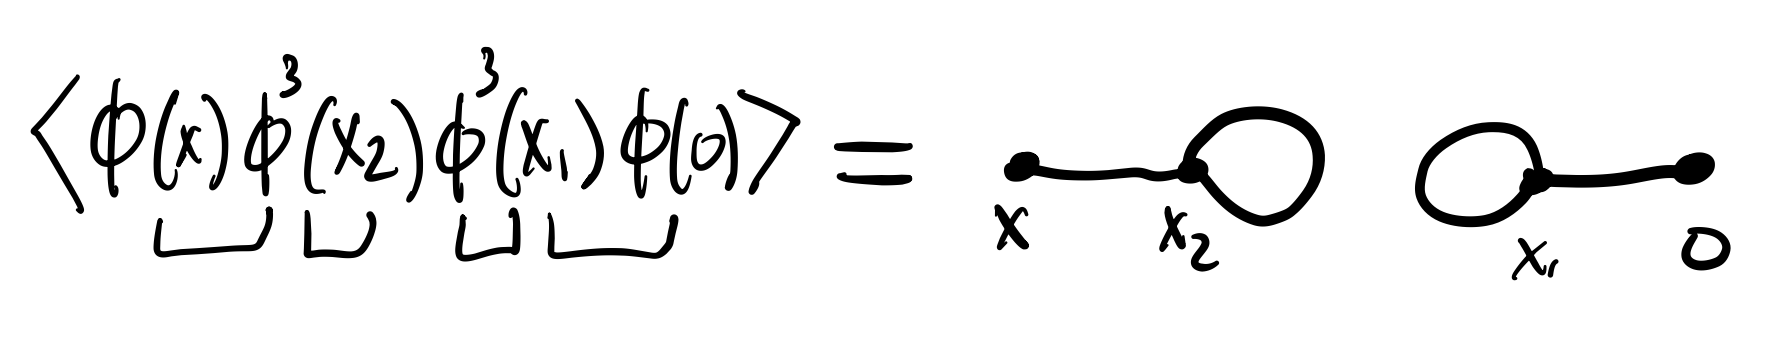
\includegraphics[scale=0.4]{Lectures/Figures/lec11-diag5.png}
\end{center}

Out of these diagrams, the last one is special. It is disconnected, i.e. there is no connection between $x$ and $0$, thus it does not depend on the distance between $x$ and $0$. It will get cancelled out when we look at the connected correlation function, as these diagrams are precisely the corrections to the one-point functions, i.e. $\avg{\phi(x)}\avg{\phi(0)}$, where the correction to $\avg{\phi(x)}$ corresponds to the left piece of the above diagram and $\avg{\phi(0)}$ corresponds to the right piece of the above diagram.

The final result is that:
\begin{equation}
    \avg{\phi(x)\phi(0)}_{\lambda, c} = \avg{\phi(x)\phi(0)}_0 + \frac{i^2}{2}\left.\avg{\phi(x)(S_{\text{int}})^2\phi(0)}\right|_{\text{no bubbles, connected}} + O(\lambda^3)
\end{equation}
and we will go through this on Thursday in more detail, getting the combinatorial factors right.